\documentclass[14pt, table]{extarticle}
\usepackage{amsfonts}
\usepackage{amsmath}
\usepackage[utf8]{inputenc}
\usepackage[a4paper, total={7in, 10.5in}]{geometry}
\usepackage[table]{xcolor}
\usepackage{tgbonum}
\usepackage{float}
\usepackage{graphicx}
\graphicspath{ {./images/} }
\DeclareGraphicsExtensions{.png,.jpg}
\usepackage{tikz}
\usepackage{circuitikz}
\usepackage[T1]{fontenc}
\usetikzlibrary{quotes,angles}
\usetikzlibrary{arrows}

\title{\textbf{Sprawozdanie} \\ \Large{Ćwiczenie 1}}
\date{Data wykonania: 15 marca 2023}
\author{ \Large{Jan Kwinta} \\ \large{Prowadzący ćwiczenia: prof. Jerzy Smyrski}}


\newcommand{\nl}{\vspace{0.5cm}}
\newcommand{\nz}{\vspace{1.5cm}}
\newcommand{\zatem}{\textrm{Zatem }}

\definecolor{trueGreen}{HTML}{009900}

\begin{document}
\maketitle

\paragraph{Wstęp teoretyczny}

\paragraph{Ćwiczenie 1.1 \\}
Obserwacja syngałów z generatora
\begin{figure}[H]
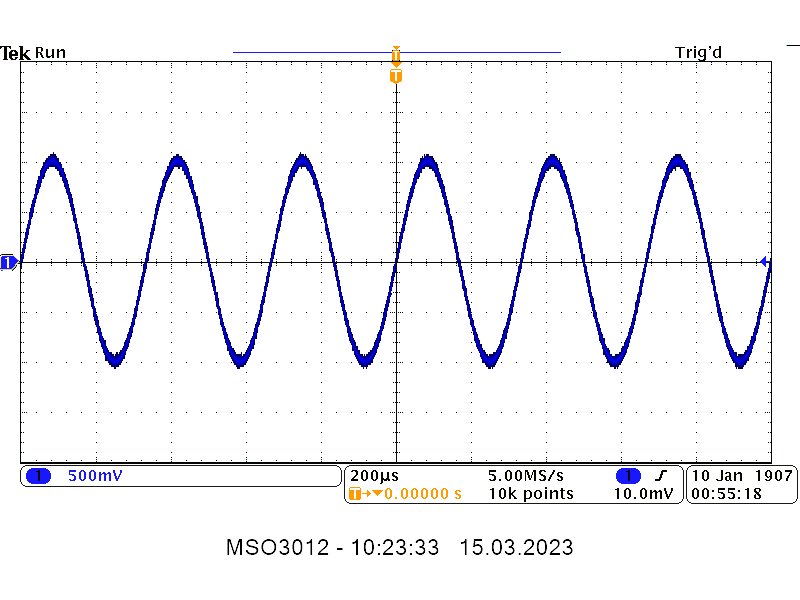
\includegraphics[scale=0.7]{A18}
\centering
\end{figure}

\begin{figure}[H]
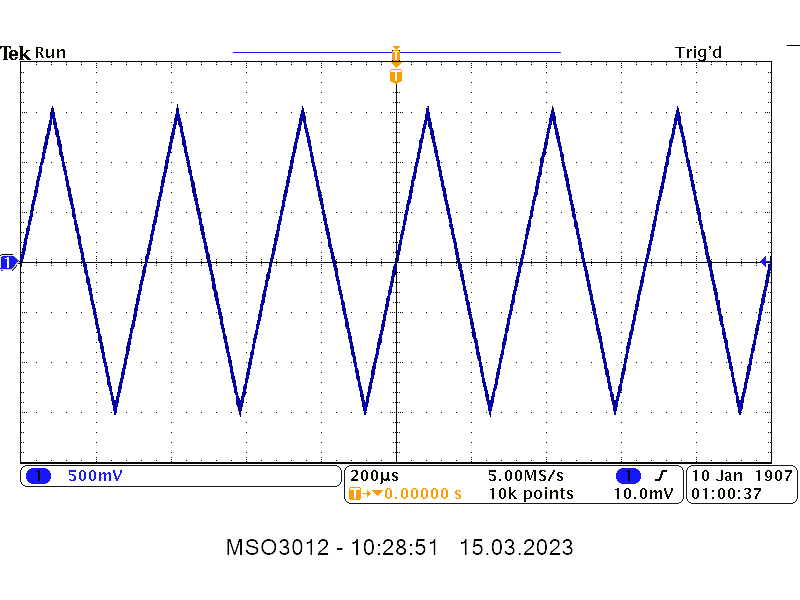
\includegraphics[scale=0.7]{A20}
\centering
\end{figure}

\begin{figure}[H]
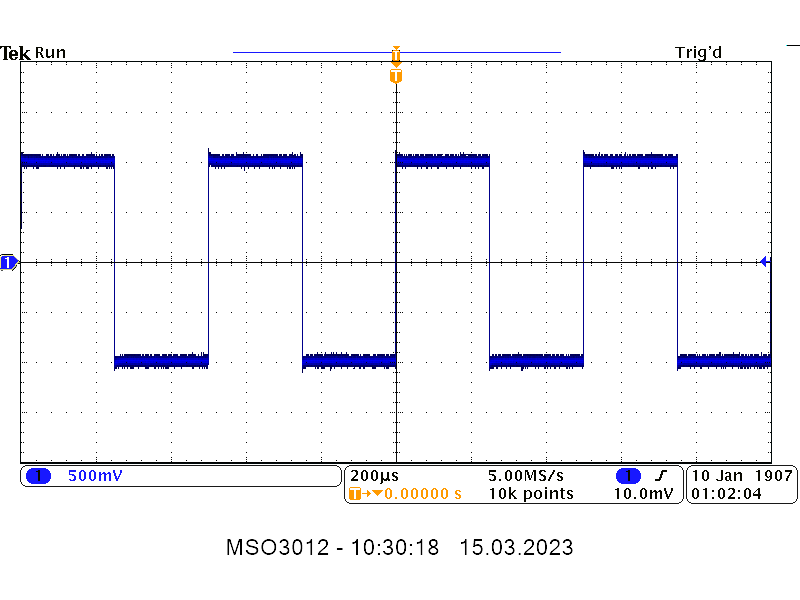
\includegraphics[scale=0.7]{A17}
\centering
\end{figure}

Pomiar amplitudy i częstotliwości sygnałów

\begin{figure}[H]
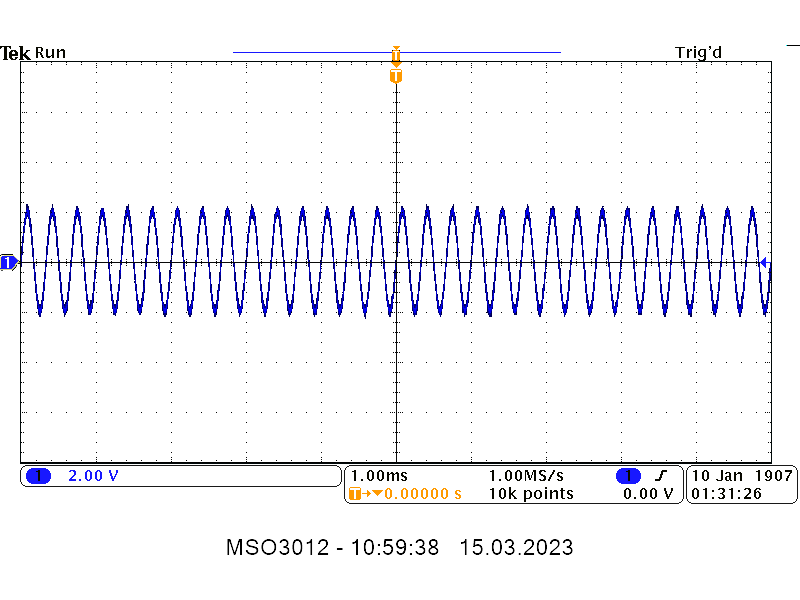
\includegraphics[scale=0.7]{A11}
\centering
\end{figure}

\begin{figure}[H]
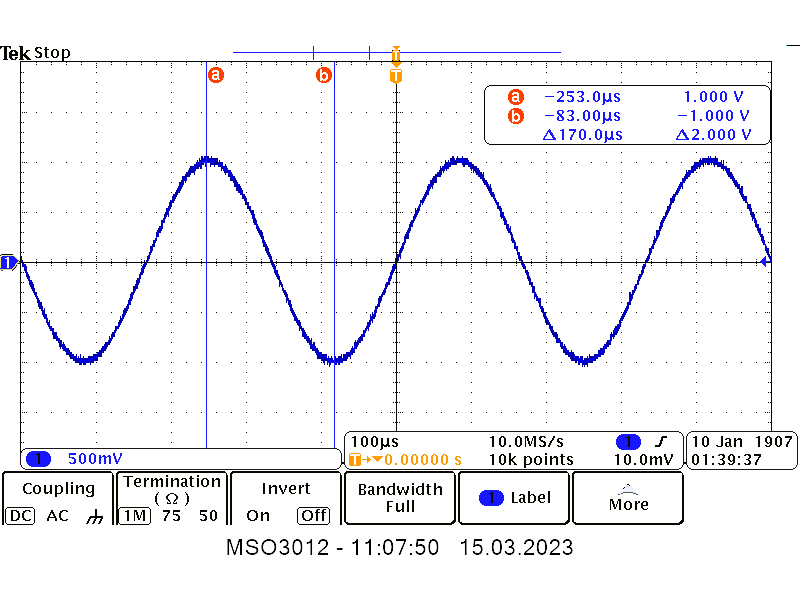
\includegraphics[scale=0.7]{A12}
\centering
\end{figure}

\begin{figure}[H]
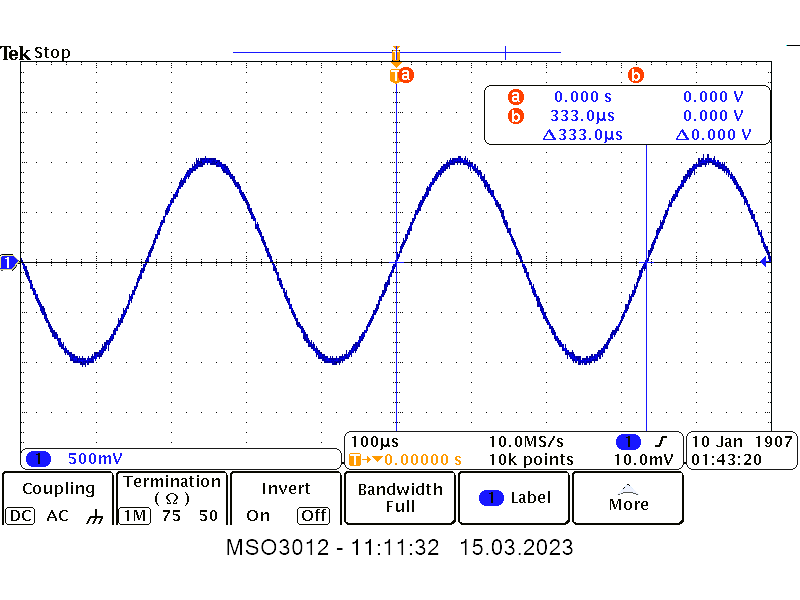
\includegraphics[scale=0.7]{A13}
\centering
\end{figure}

\begin{figure}[H]
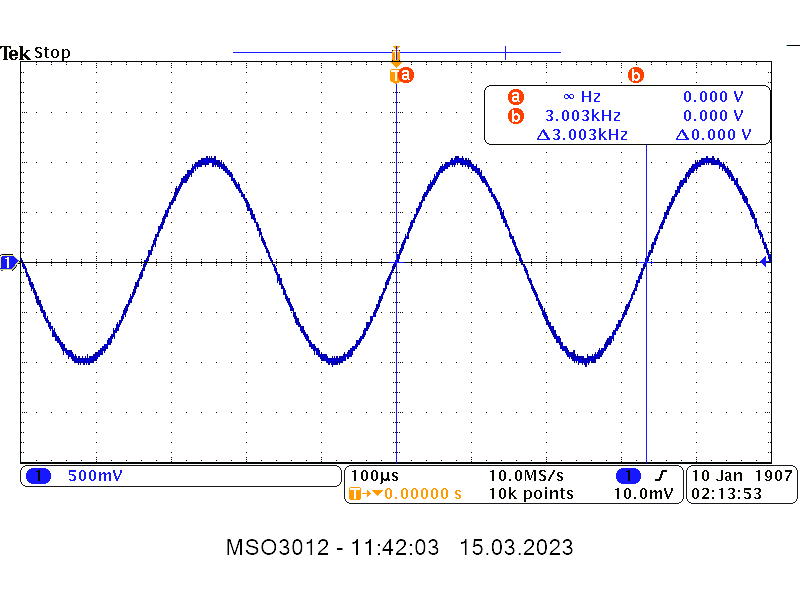
\includegraphics[scale=0.7]{A14}
\centering
\end{figure}

\begin{figure}[H]
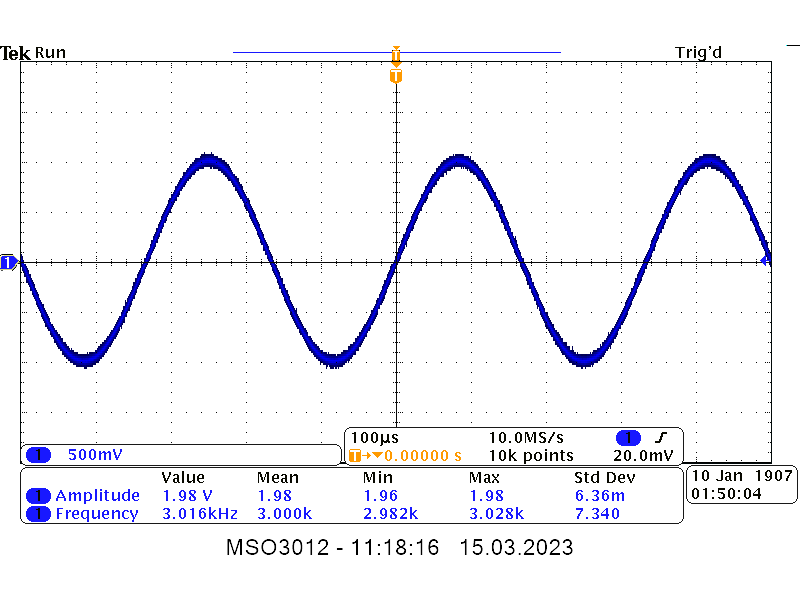
\includegraphics[scale=0.7]{A15}
\centering
\end{figure}

Pomiar przesunięcia fazy
\begin{figure}[H]
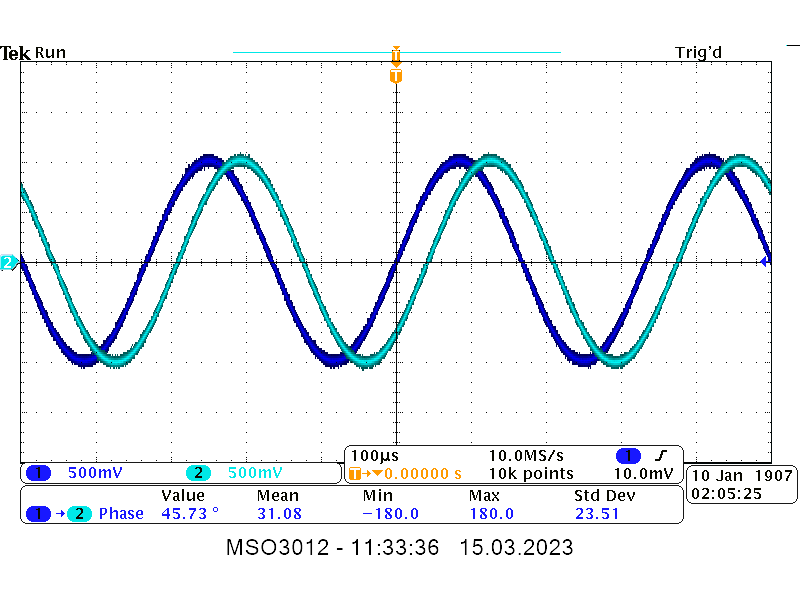
\includegraphics[scale=0.7]{A4}
\centering
\end{figure}

\paragraph{Ćwiczenie 1.2 \\}
Krzywe Lissajousa

\begin{figure}[H]
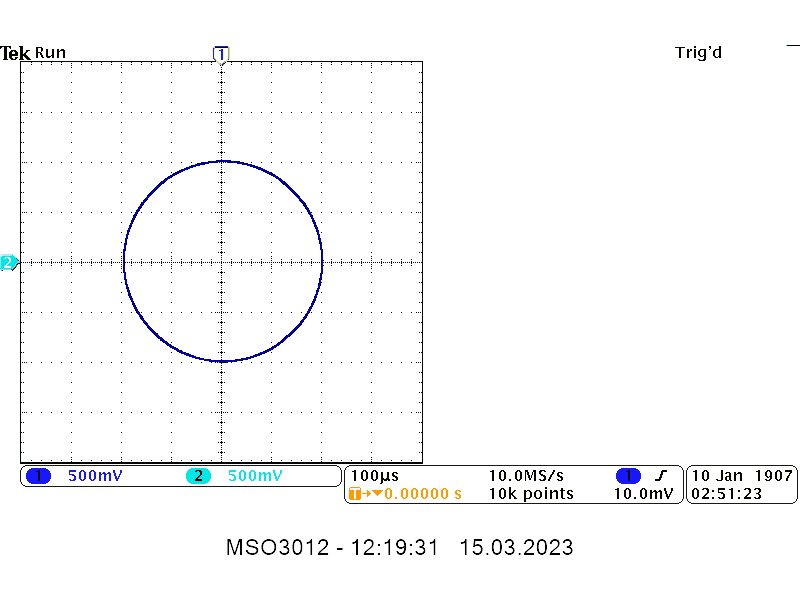
\includegraphics[scale=0.7]{A9}
\centering
\end{figure}

\begin{figure}[H]
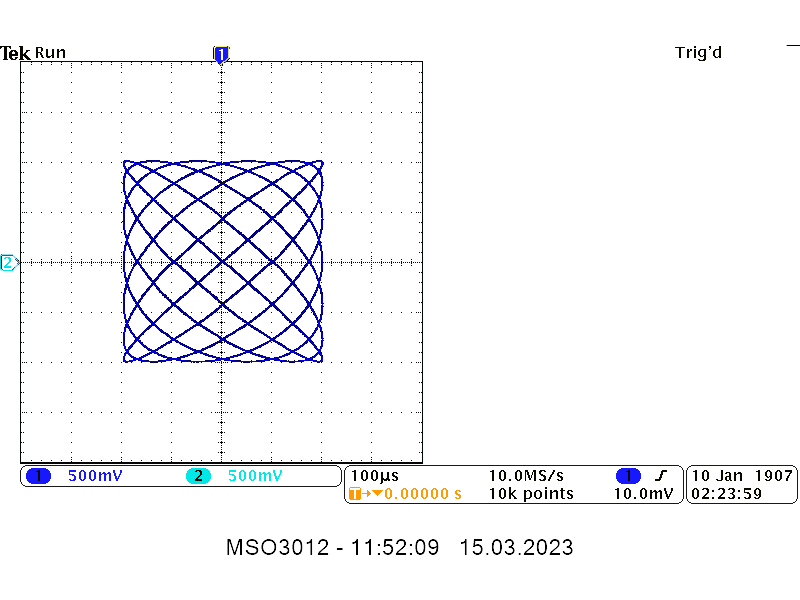
\includegraphics[scale=0.7]{A5}
\centering
\end{figure}

\begin{figure}[H]
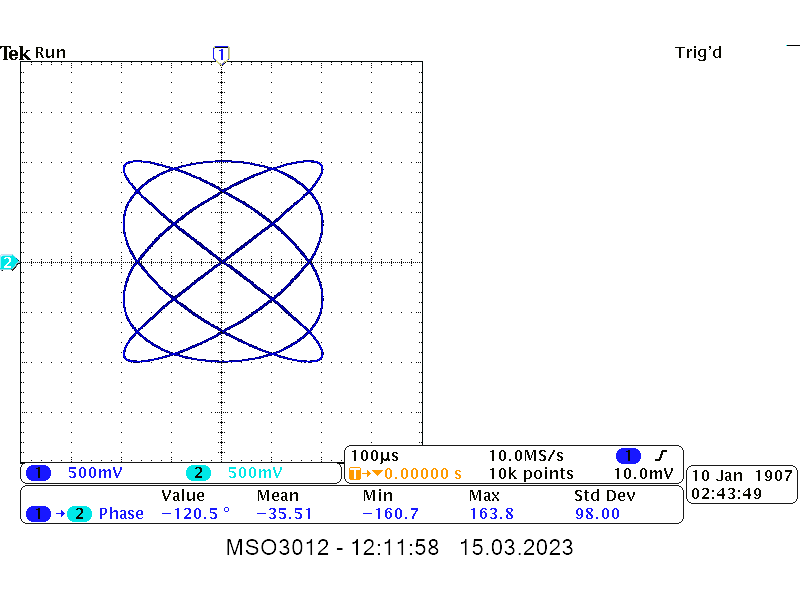
\includegraphics[scale=0.7]{A6}
\centering
\end{figure}

\begin{figure}[H]
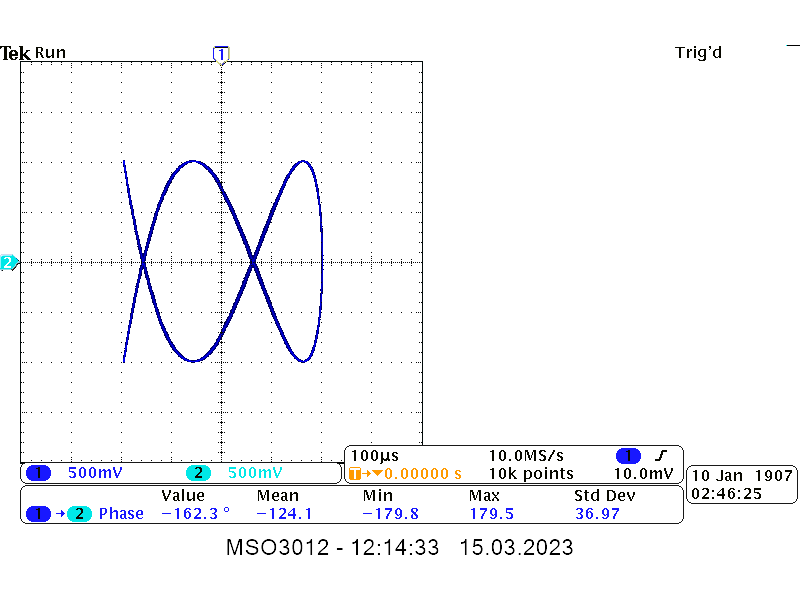
\includegraphics[scale=0.7]{A7}
\centering
\end{figure}

\begin{figure}[H]
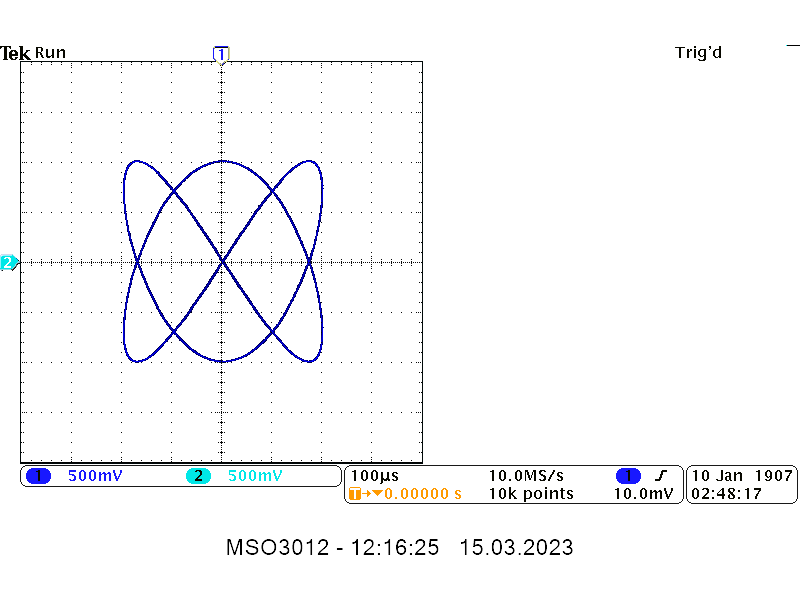
\includegraphics[scale=0.7]{A8}
\centering
\end{figure}

\begin{figure}[H]
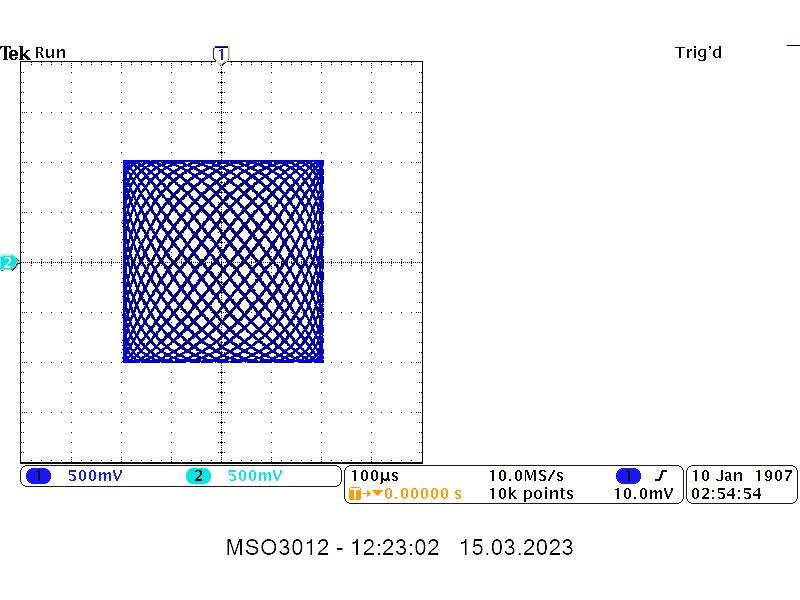
\includegraphics[scale=0.7]{A10}
\centering
\end{figure}

\paragraph{Ćwiczenie 1.3 \\}
Dudnienia 
\begin{figure}[H]
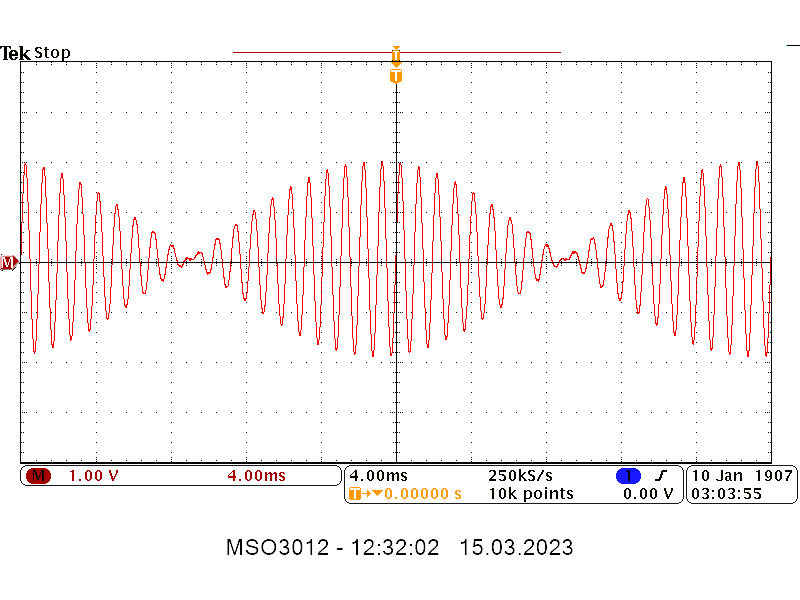
\includegraphics[scale=0.7]{A0}
\centering
\end{figure}

\begin{figure}[H]
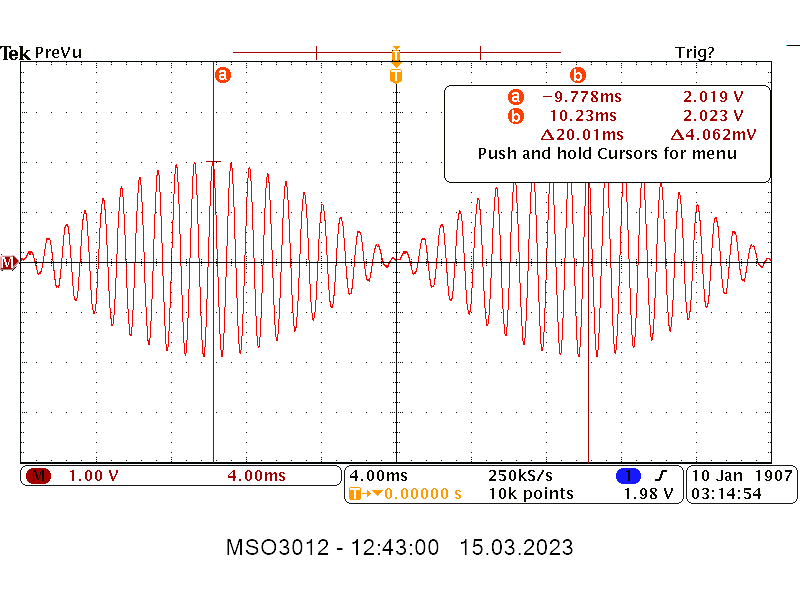
\includegraphics[scale=0.7]{A2}
\centering
\end{figure}

\begin{figure}[H]
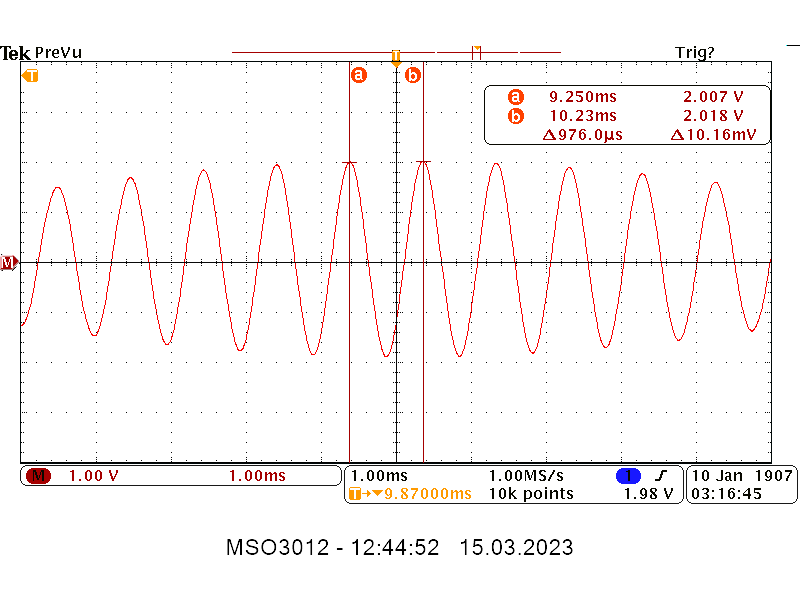
\includegraphics[scale=0.7]{A3}
\centering
\end{figure}




\paragraph{Omówienie wyników}

\paragraph{Podsumowanie}
\newpage
\paragraph{Notatki z zeszytu labolatoryjnego}
Poniżej załączone są notatki z zeszytu labolatoryjnego, które prowadziłem podczas zajęć wykonując pomiary

\begin{figure}[H]
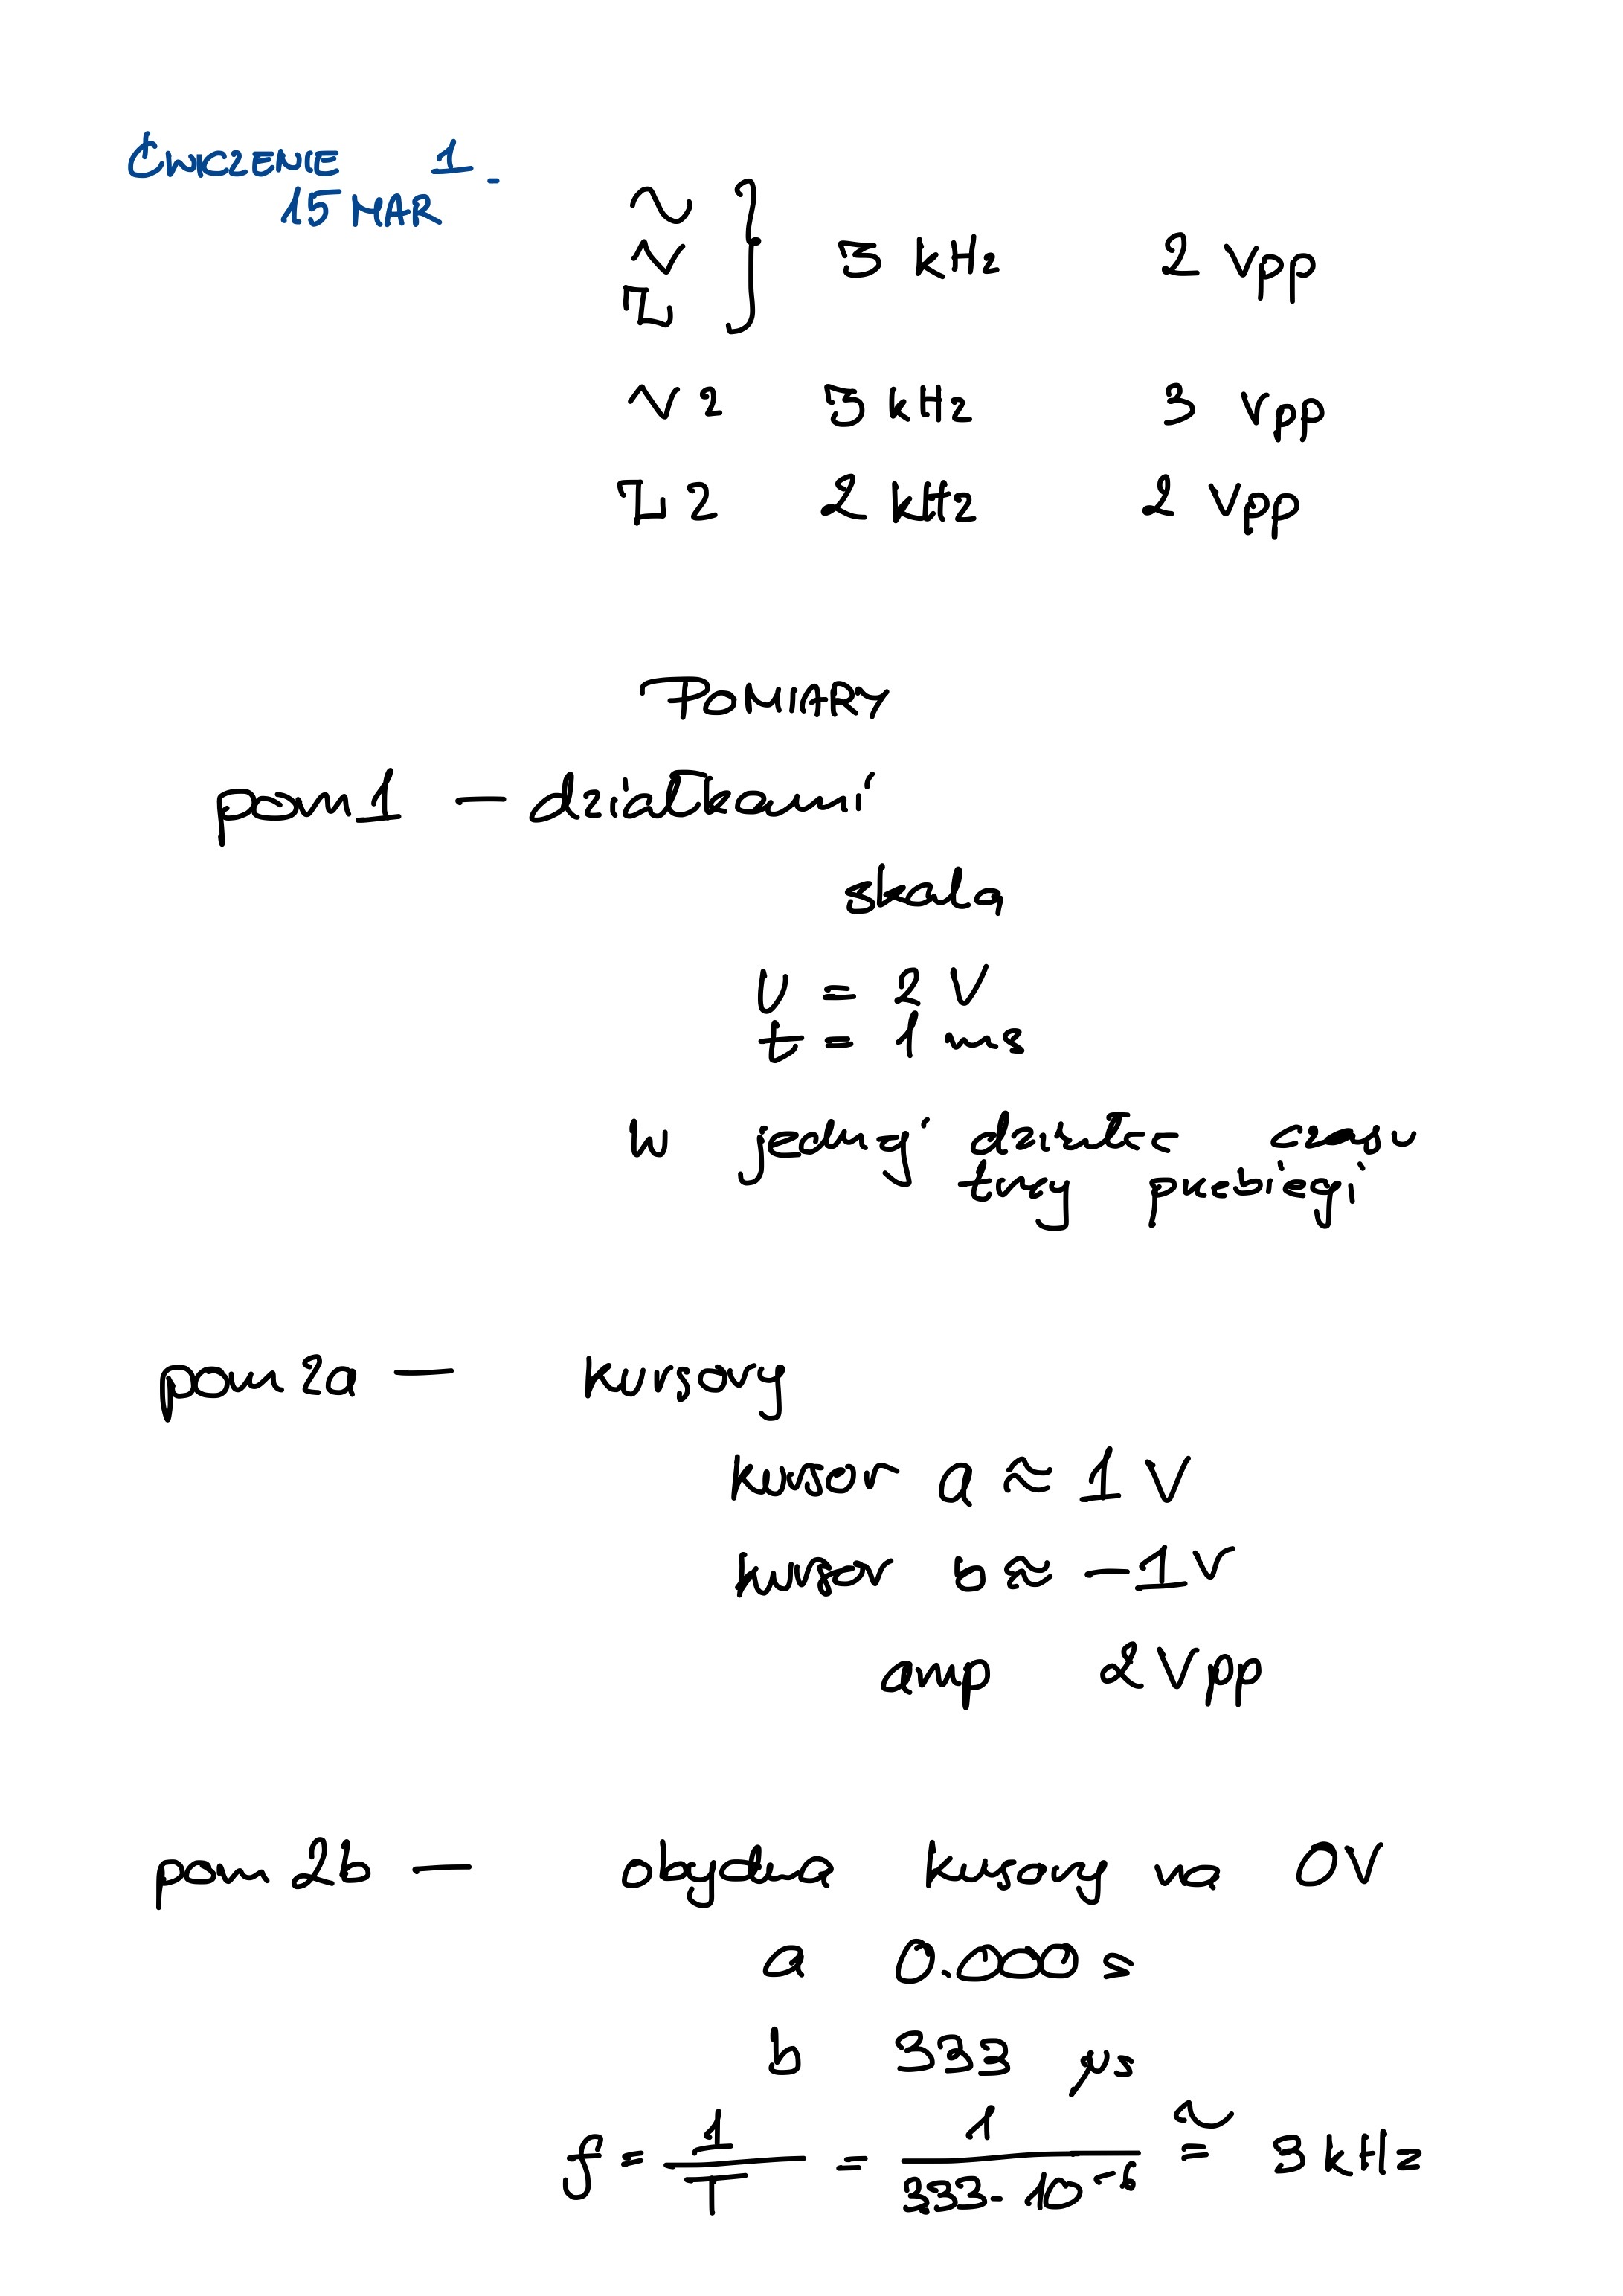
\includegraphics[scale=0.23]{B0}
\centering
\end{figure}

\begin{figure}[H]
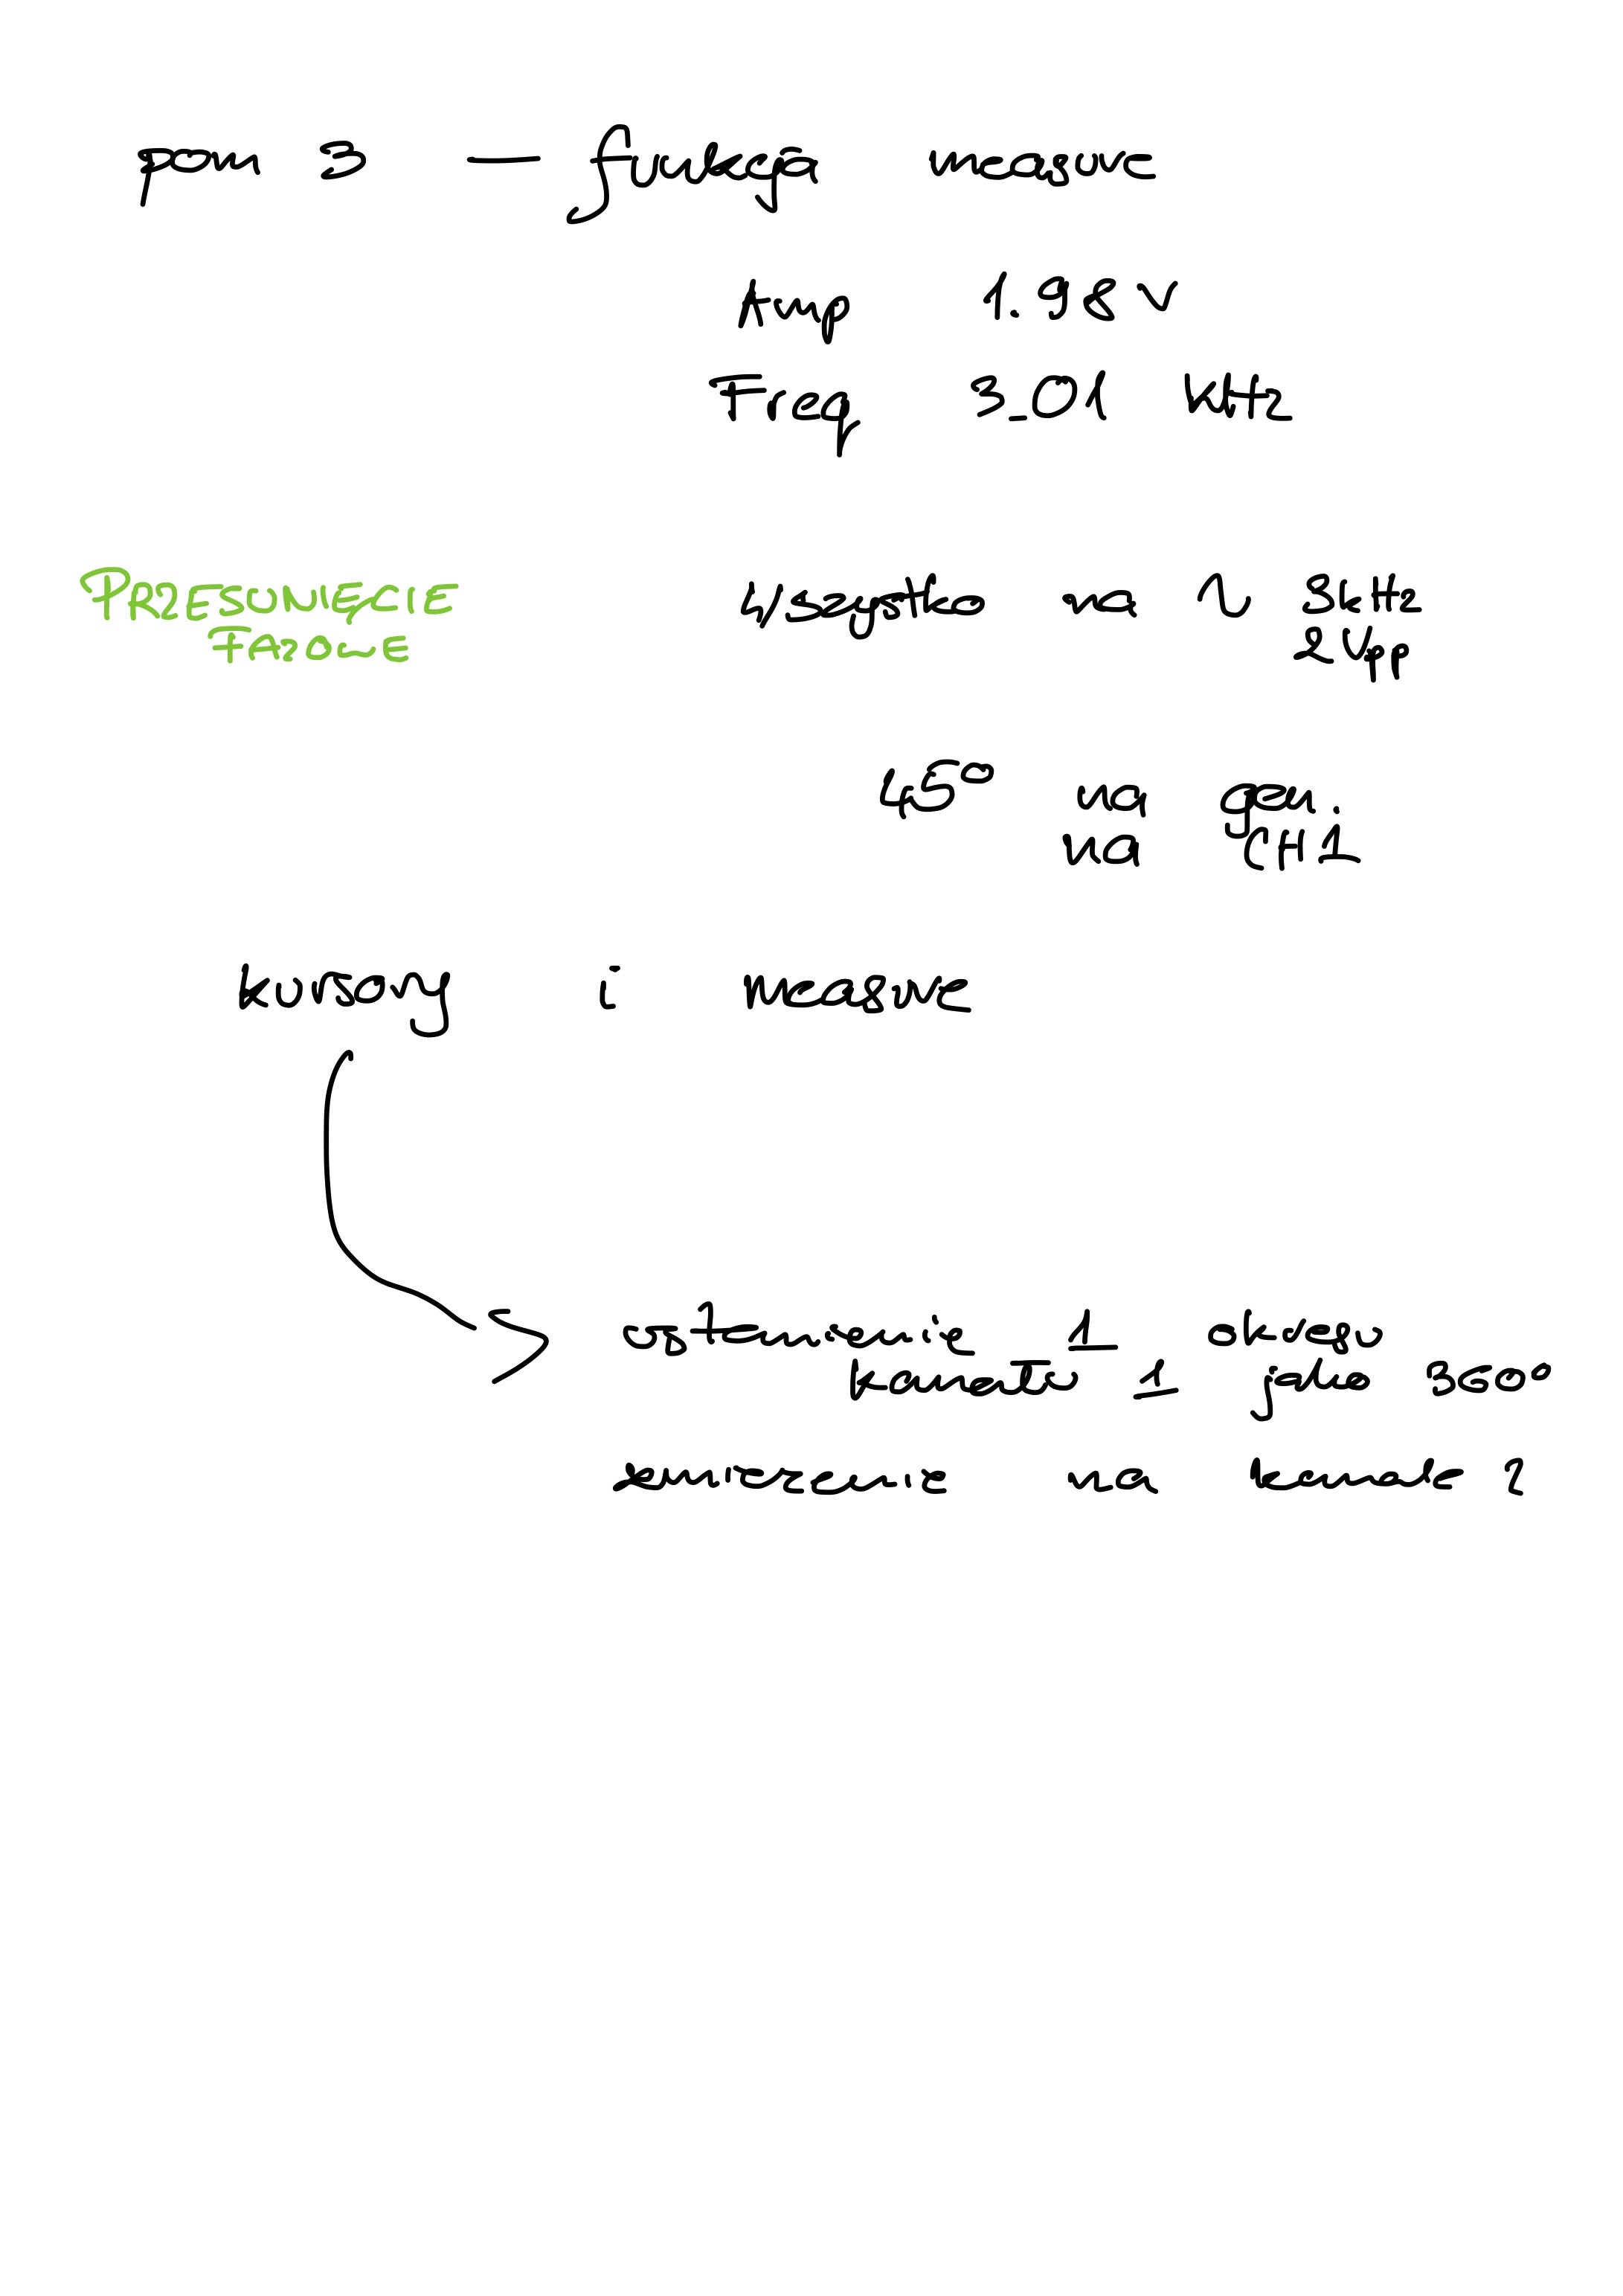
\includegraphics[scale=0.23]{B1}
\centering
\end{figure}

\begin{figure}[H]
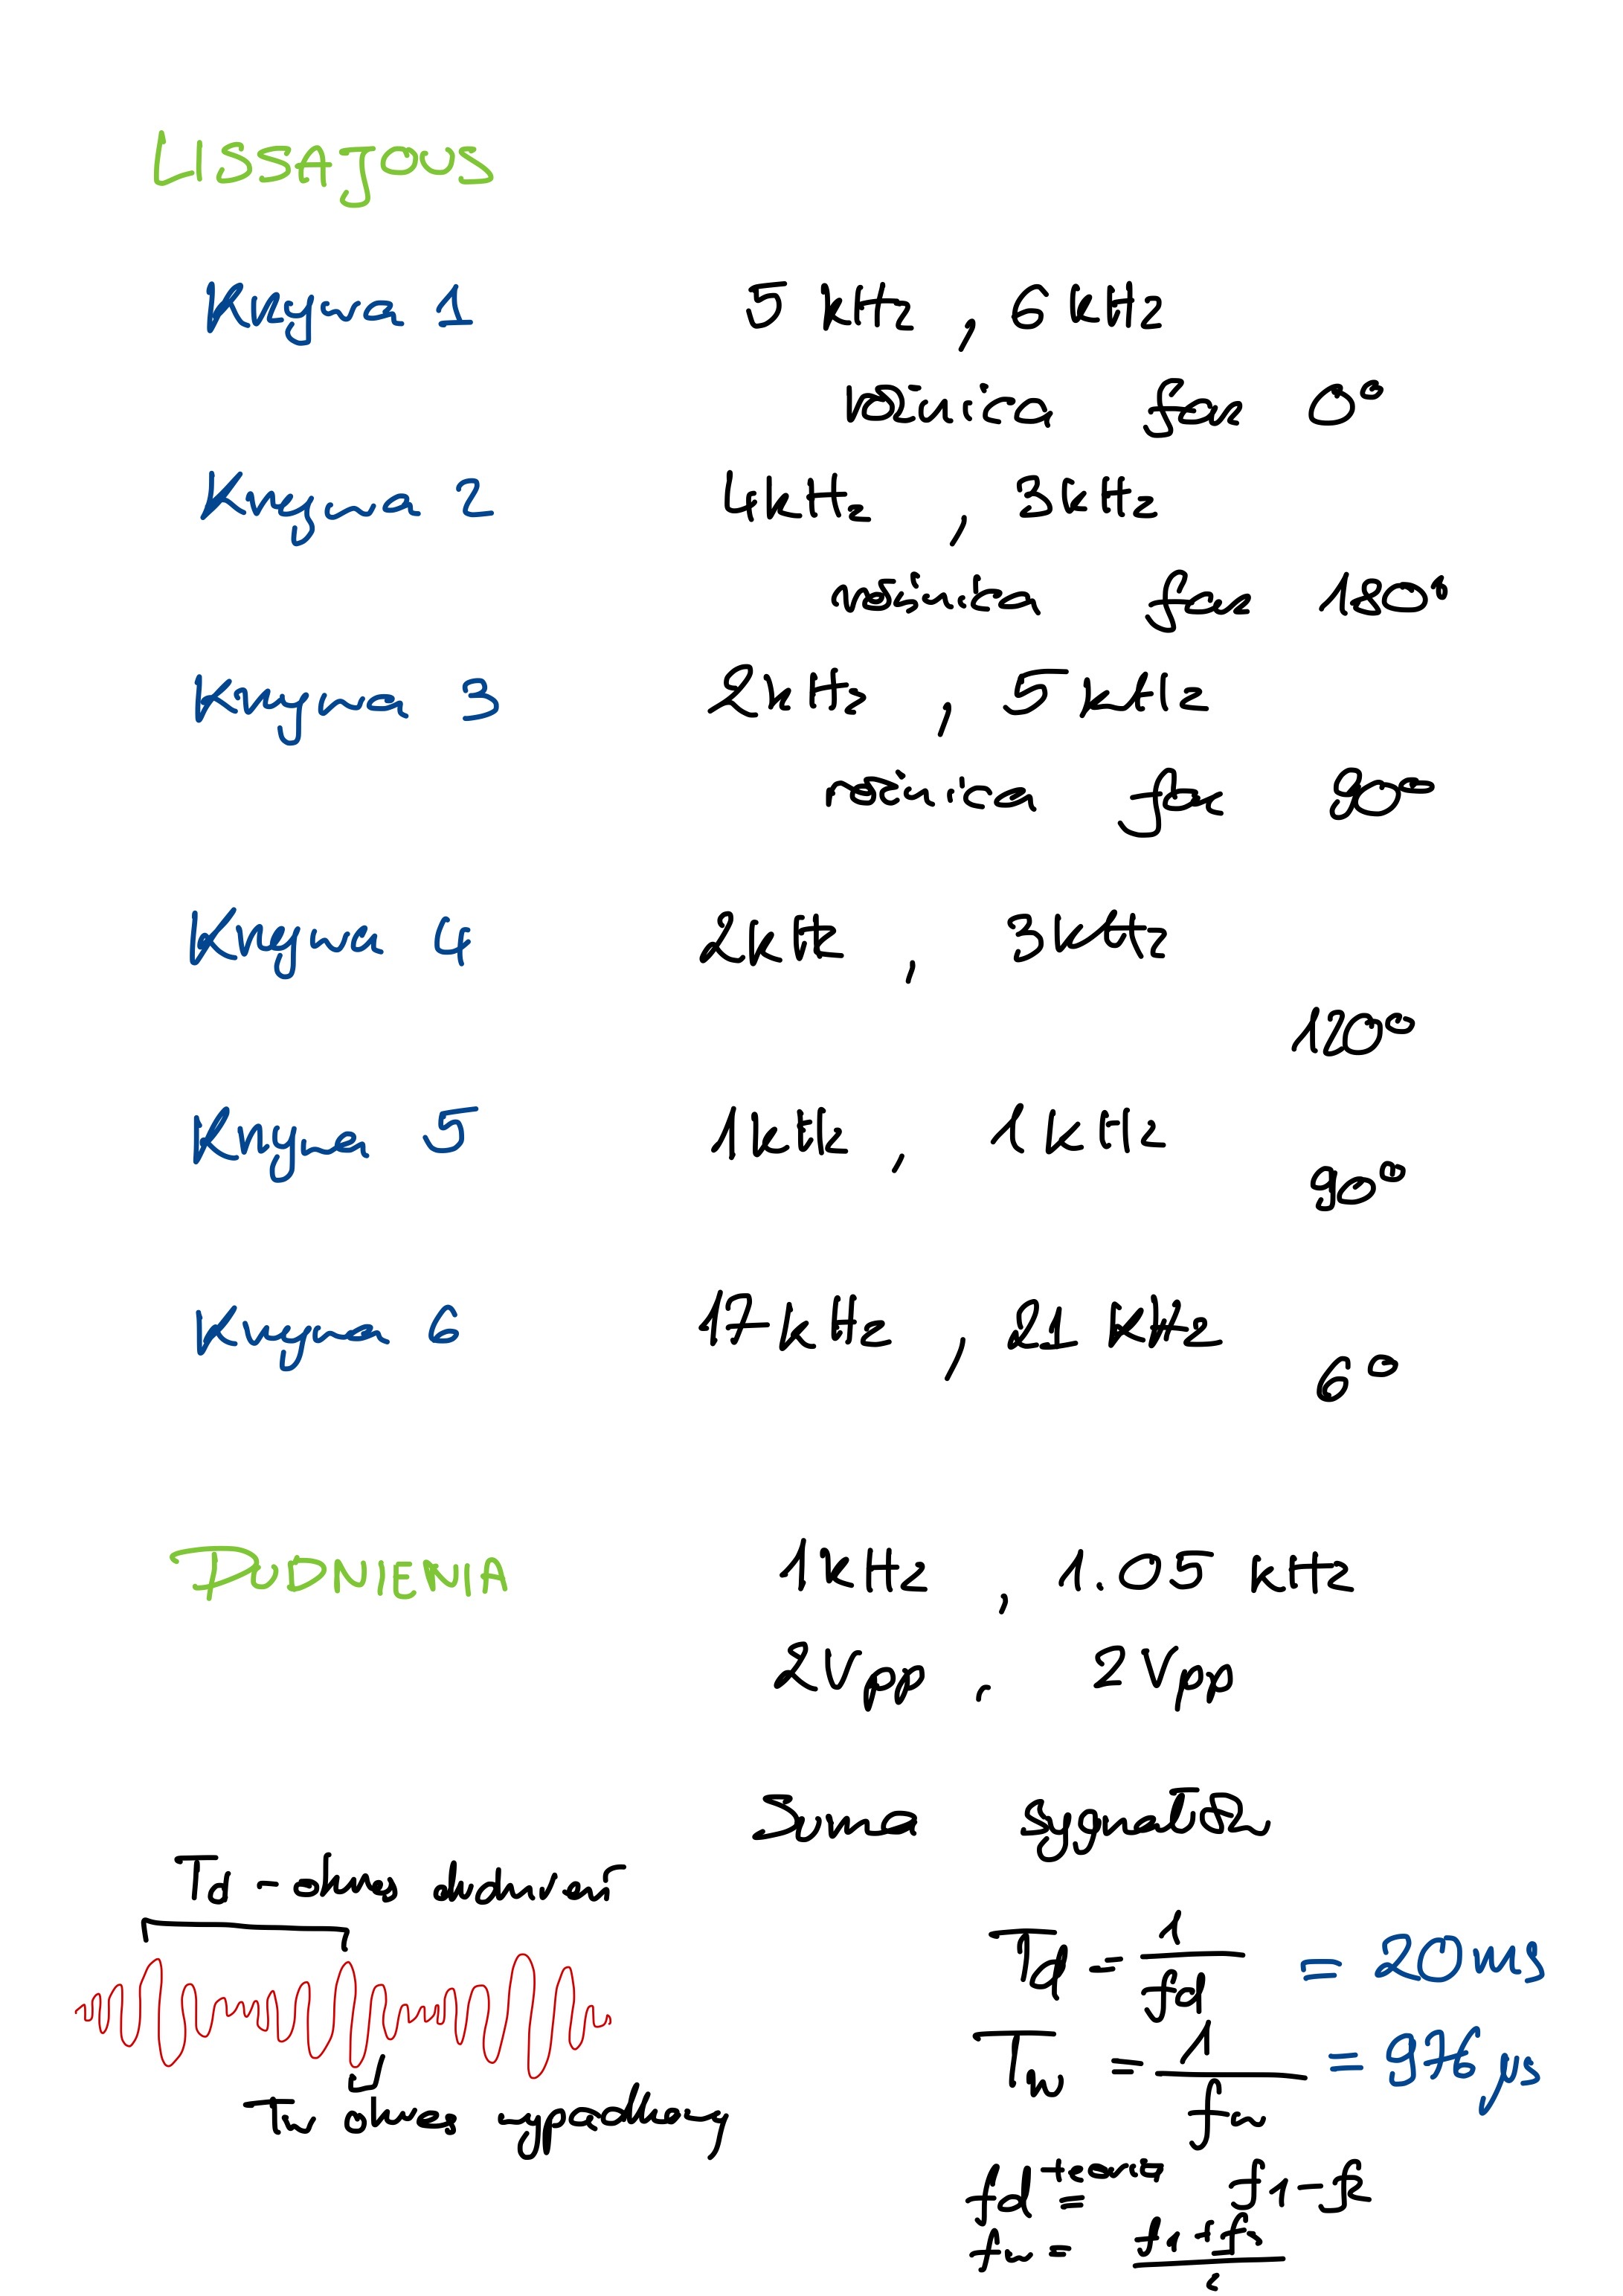
\includegraphics[scale=0.23]{B2}
\centering
\end{figure}

\end{document}